\scanpage{5}
\mspage{1}
% archive sheet number: 4
\deleted{\unsure{219|29}}

\uline{5 juillet} L'affaire a tendance à s'enliser, et j'ai envie de tout reprendre, d'une façon \deleted{\unsure{critique}} un peu différente.

\unsure{N} Si $L$ est un ensemble ordonné, je lui associe la maquette \deleted{\unsure{A}}
\[
\unsure{\mathscr M|\mathcal M}=\mathscr M_0\amalg\mathscr M_1
\]
\inserted{$I_{a,b}$}
\[
\begin{aligned}
\mathscr M_0&=L,\quad\text{ensemble des ``\uline{sommets}'' virtuels, ou ``\uline{lieux}''.}\\
\mathscr M_1&\unsure{\overset{\mathrm{d\acute ef}}{=}}\operatorname{Drap}_2(L).
\end{aligned}
\]
Si $\{a,b\}$ $(a<b)$ est un $\operatorname{Drap}_2(L)$, je note $I_{\{a,b\}}$ ou $I_{a,b}$ ou $I_{b,a}$ la strate associée, appelée aussi \uline{intervalle} déterminé par $\{a,b\}$.
% slanted
\margin{On suppose $L$ connexe, $\operatorname{card}L\geq2$.}

\deleted{Relation d'incidence : $X\triangleleft Y$ ssi $X\in$}

Notation $\partial X$, $X\in\mathscr M$ :
\[
\text{\textcircled{a}}\quad
\begin{cases}
\partial I_{\{a,b\}}=\{a,b\}\subset\mathscr M_0\\
\partial x=\varnothing\subset\mathscr M
\end{cases}
\qquad
\text{\textcircled{b}}\quad
\begin{cases}
\delta I_{a,b}=\partial I_{a,b}=\{a,b\}\\
\delta x=\{x\}
\end{cases}
\]
% slanted
\margin{support ``naïf''\par
$c\ \left\{\begin{aligned}|I_{a,b}|^{\unsure{\circ}}&=[a,b]=\{x\in L\mid a\leq x\unsure{\leq b}\}\\|a|&=\{a\}\end{aligned}\right.$\par
$d)\quad |X|^\circ=|X|\setminus\partial X\ \begin{cases}]a,b[&\text{si }X=\unsure{I_{a,b}}\\\{a\}&\text{si }X=a\end{cases}$\par
Notons, pour $X\in\mathscr M$, $\delta X$ et $\partial X\subset L$, mais $\partial X\subset\delta X$.}

\uline{Relation d'incidence :} $X\triangleleft Y$ ssi $X\unsure{\equiv|=}x\in L$, $Y\in\mathscr M_1$, et $x\in\partial Y$. Donc la notion $\partial X$ du début est celle associée à cette relation d'incidence
\[
\partial X=\{Y\in\mathscr M\mid Y\triangleleft X\}\qquad(X\in\mathscr M)
\]
[Il semble qu'il soit mieux introduire d'abord la relation $\leq$ sur $\mathscr M$, d'interpréter $\deleted{\unsure{I_{a,b}}}$, $I_{a,b}^\circ$, $I_{<a}$, $I_{>b}$ comme des ``intervalles'' de $\mathscr M$, i.e. les \unsure{sous-ensembles} via $\unsure{\mathrm{Ord}^\circ}$.]

Relation $\ll$. On a par définition
\[
X\overset{\circ}{\ll}Y\Longleftrightarrow |X|\subset|Y|\quad\text{et}\quad\deleted{\unsure{X\ne Y}}\ X\overline{\triangleleft}Y.
\]
\[
X\overset{\circ}{\ll}Y\Longleftrightarrow
\begin{cases}
X=Y\\
\text{ou }X=x\in L,\ Y=I_{a,b},\quad a<x<b\\
\text{ou }X=I_{a,b},\ Y=I_{a',b'},\quad a'\leq a<b\leq b'
\end{cases}
\]
\margin{\figure{\begin{tikzpicture}
\node[anchor=north west,inner sep=1pt,text width=\marginparwidth,align=left] (note) at (0,0) {Relat\textsuperscript{n} d'ordre\par\uline{Maq $2,\deleted{\unsure{4}}$OK}};
\draw[gray] ([xshift=-2mm,yshift=2mm]note.north west) .. controls ([xshift=8mm,yshift=3mm]note.north west) and ([xshift=-6mm,yshift=3mm]note.north east) .. ([xshift=2mm,yshift=0mm]note.north east) -- ([xshift=2mm,yshift=-2mm]note.south east) .. controls ([xshift=-6mm,yshift=-2mm]note.south east) and ([xshift=6mm,yshift=-2mm]note.south west) .. ([xshift=-2mm,yshift=-2mm]note.south west);
\end{tikzpicture}}}

\figure{\begin{tikzpicture}
\node[anchor=north west,inner sep=0pt] (body) at (0,0) {\begin{minipage}{.86\linewidth}
\uline{Remarque}\quad
$X\overset{\deleted{\unsure{\circ}}}{\ll}Y\Longrightarrow\delta X\cup\delta Y\in\operatorname{Drap}(L)$

\uline{Conséquence}\quad Relation $X\overset{\deleted{\unsure{\circ}}}{\ll}Y$ $(\overset{\mathrm{d\acute ef}}{\Longleftrightarrow}\exists Y',\ X\overset{\circ}{\ll}Y'\unsure{\unlhd|\trianglelefteq} Y)$
\[
\begin{aligned}
X\ll Y&\Longleftrightarrow\deleted{\unsure{X=Y}}\ \text{ou}\ \underbrace{X\triangleleft Y\ \text{ou}\ X\overset{\circ}{\ll}Y}_{\text{\deleted{\unsure{mut}}mutuellement exclusifs}}\Longleftrightarrow|X|\subset|Y|\\
&\Longleftrightarrow\begin{cases}
X=Y\\
\text{ou }X=x\in L,\ Y=I_{a,b},\quad a\leq x\leq b\\
\text{ou }X=I_{a,b},\ Y=I_{a',b'},\quad a'\leq\unsure{a}<b\leq b'
\end{cases}
\end{aligned}
\]
\end{minipage}};
\draw[gray] ([xshift=2mm,yshift=4mm]body.north west) .. controls ([xshift=-7mm,yshift=5mm]body.north west) and ([xshift=-7mm,yshift=-9mm]body.north west) .. ([xshift=1mm,yshift=-8mm]body.north west);
\draw[gray,->] ([xshift=-4mm,yshift=-6mm]body.north west) .. controls ([xshift=-11mm,yshift=-13mm]body.north west) and ([xshift=-11mm,yshift=5mm]body.south west) .. ([xshift=-7mm,yshift=-1mm]body.south west) .. controls ([xshift=-5mm,yshift=-6mm]body.south west) and ([xshift=6mm,yshift=-6mm]body.south west) .. ([xshift=12mm,yshift=-6mm]body.south west);
\end{tikzpicture}}
